\subsection{Vector data}

\begin{figure}[htb]
  \centering
  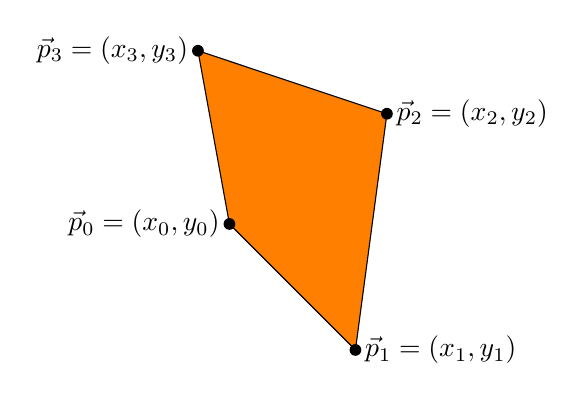
\begin{tikzpicture}[scale=2]
  \coordinate (zero) at (0, 0);
  \coordinate (one) at (0.8, -0.8);
  \coordinate (two) at (1, 0.7);
  \coordinate (three) at (-0.2, 1.1);
  \draw[fill=orange]
    (zero) node[left] {$\vec{p}_0 = (x_0, y_0)$}
    -- (one) node[right] {$\vec{p}_1 = (x_1, y_1)$}
    -- (two) node[right] {$\vec{p}_2 = (x_2, y_2)$}
    -- (three) node[left] {$\vec{p}_3 = (x_3, y_3)$}
    -- cycle;
  \foreach \n in {zero,one,two,three}
    \node at (\n)[circle,fill,inner sep=1.5pt]{};
\end{tikzpicture}

  \textcolor{gray}{\vrule}
  \hspace{0.01\linewidth}
  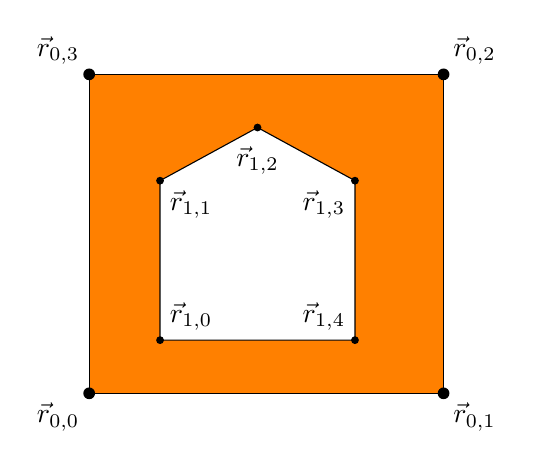
\begin{tikzpicture}[scale=2.25]
  \coordinate (zero) at (0, 0);
  \coordinate (one) at (2.0, 0);
  \coordinate (two) at (2.0, 1.8);
  \coordinate (three) at (0, 1.8);
  \draw[fill=orange]
    (zero) node[below left] {$\vec{r}_{0,0}$}
    -- (one) node[below right] {$\vec{r}_{0,1}$}
    -- (two) node[above right] {$\vec{r}_{0,2}$}
    -- (three) node[above left] {$\vec{r}_{0,3}$}
    -- cycle;
  \foreach \n in {zero,one,two,three}
    \node at (\n)[circle,fill,inner sep=1.5pt]{};

  \coordinate (0) at (0.4, 0.3);
  \coordinate (1) at (1.5, 0.3);
  \coordinate (2) at (1.5, 1.2);
  \coordinate (3) at (0.95, 1.5);
  \coordinate (4) at (0.4, 1.2);
  \draw[fill=white]
    (0) node[above right] {$\vec{r}_{1,0}$}
    -- (1) node[above left] {$\vec{r}_{1,4}$}
    -- (2) node[below left] {$\vec{r}_{1,3}$}
    -- (3) node[below=3.5pt] {$\vec{r}_{1,2}$}
    -- (4) node[below right] {$\vec{r}_{1,1}$}
    -- cycle;
  \foreach \n in {0,1,2,3,4}
    \node at (\n)[circle,fill,inner sep=1pt]{};
\end{tikzpicture}

  \caption{
    Simple polygon with four unique vertices is shown on the left hand side.
    A complex polygon with an an outer hull (shown in \textbf{black})
    and an interior hull (shown \textcolor{orange}{\textbf{orange}}) is shown on the right hand side for comparison.
  }
\end{figure}

\begin{figure}[H]
  \centering
  \begin{tikzpicture}[scale=1]
  \coordinate (ll) at (0, 0);
  \coordinate (mid) at (2, 1);
  \coordinate (lr) at (4, 0);
  \coordinate (ur) at (4, 2);
  \coordinate (ul) at (0, 2);
  \draw[fill=orange]
    (ll) node[left] {$\vec{r}_0$}
    -- (ur) node[right] {$\vec{r}_1$}
    -- (lr) node[right] {$\vec{r}_2$}
    -- (ul) node[left] {$\vec{r}_3$}
    -- cycle;
  \foreach \n in {ll,ur,lr,ul}
    \node at (\n)[circle,fill,inner sep=1.5pt]{};

   \draw (4.4, 1) edge[->, thick] node[above] {\texttt{buffer(0.0)}} (6.6, 1);

  \coordinate (offset) at (7, 0);
  \draw[fill=orange]
    ($ (ll) + (offset) $) node[left] {$\vec{r}_0$}
    -- ($ (mid) + (offset) $) node[below] {$\vec{r}_1$}
    -- ($ (lr) + (offset) $) node[right] {$\vec{r}_2$}
    -- ($ (ur) + (offset) $) node[right] {$\vec{r}_3$}
    -- ($ (mid) + (offset) $) node[above] {$\vec{r}_4$}
    -- ($ (ul) + (offset) $) node[left] {$\vec{r}_5$}
    -- cycle;
  \foreach \n in {ll,mid,lr,ur,mid,ul}
    \node at ($ (\n) + (offset) $)[circle,fill,inner sep=1.5pt]{};
\end{tikzpicture}

  \caption{Zero-buffering the polygon fixes self-intersecting polygons, as is shown here.}
\end{figure}
